\documentclass[10pt]{article}
% for pdflatex
\usepackage[utf8]{inputenc}
% for hyperlink
\usepackage{hyperref}
% for custom enum
\usepackage{enumitem}
% for removing alinea begin of paragraph
\usepackage{parskip}
\usepackage{array, xcolor, graphicx}
\usepackage[a4paper, margin=1cm]{geometry}
 
\title{\bfseries\Huge Ingénieur Blockchain \vspace{-4ex}}
% no author
\author{\bfseries\Huge \vspace{-4ex}}
% no date
\date{}
% custom for column style
\definecolor{lightgray}{gray}{0.8}
% custom for column type
\newcolumntype{L}{p{0.18\textwidth}}
% custom for column type
\newcolumntype{R}{p{0.75\textwidth}}
% custom for column type
\newcommand\VRule{\color{lightgray}\vrule width 2pt}
% for bullet point outside of list
\newcommand{\tabitem}{~~\llap{$\rightarrow$}~~}
\begin{document}
\begin{minipage}[t]{0.80\textwidth}
Mohamed Amine LEGHERABA\\
24 ans\\
92 bis rue Rouget de Lisle, Bezons, France\\
+33 (0) 6 30 82 90 00\\
\href{mailto:mlegheraba@protonmail.com}{mlegheraba@protonmail.com}\\
\url{https://github.com/MohamedLEGH} \\

{\bf Français}: langue maternelle \\
{\bf Anglais}: bon niveau (TOIEC: 935) \\
\end{minipage}
\begin{minipage}[t]{0.20\textwidth}
\vspace{-3ex}
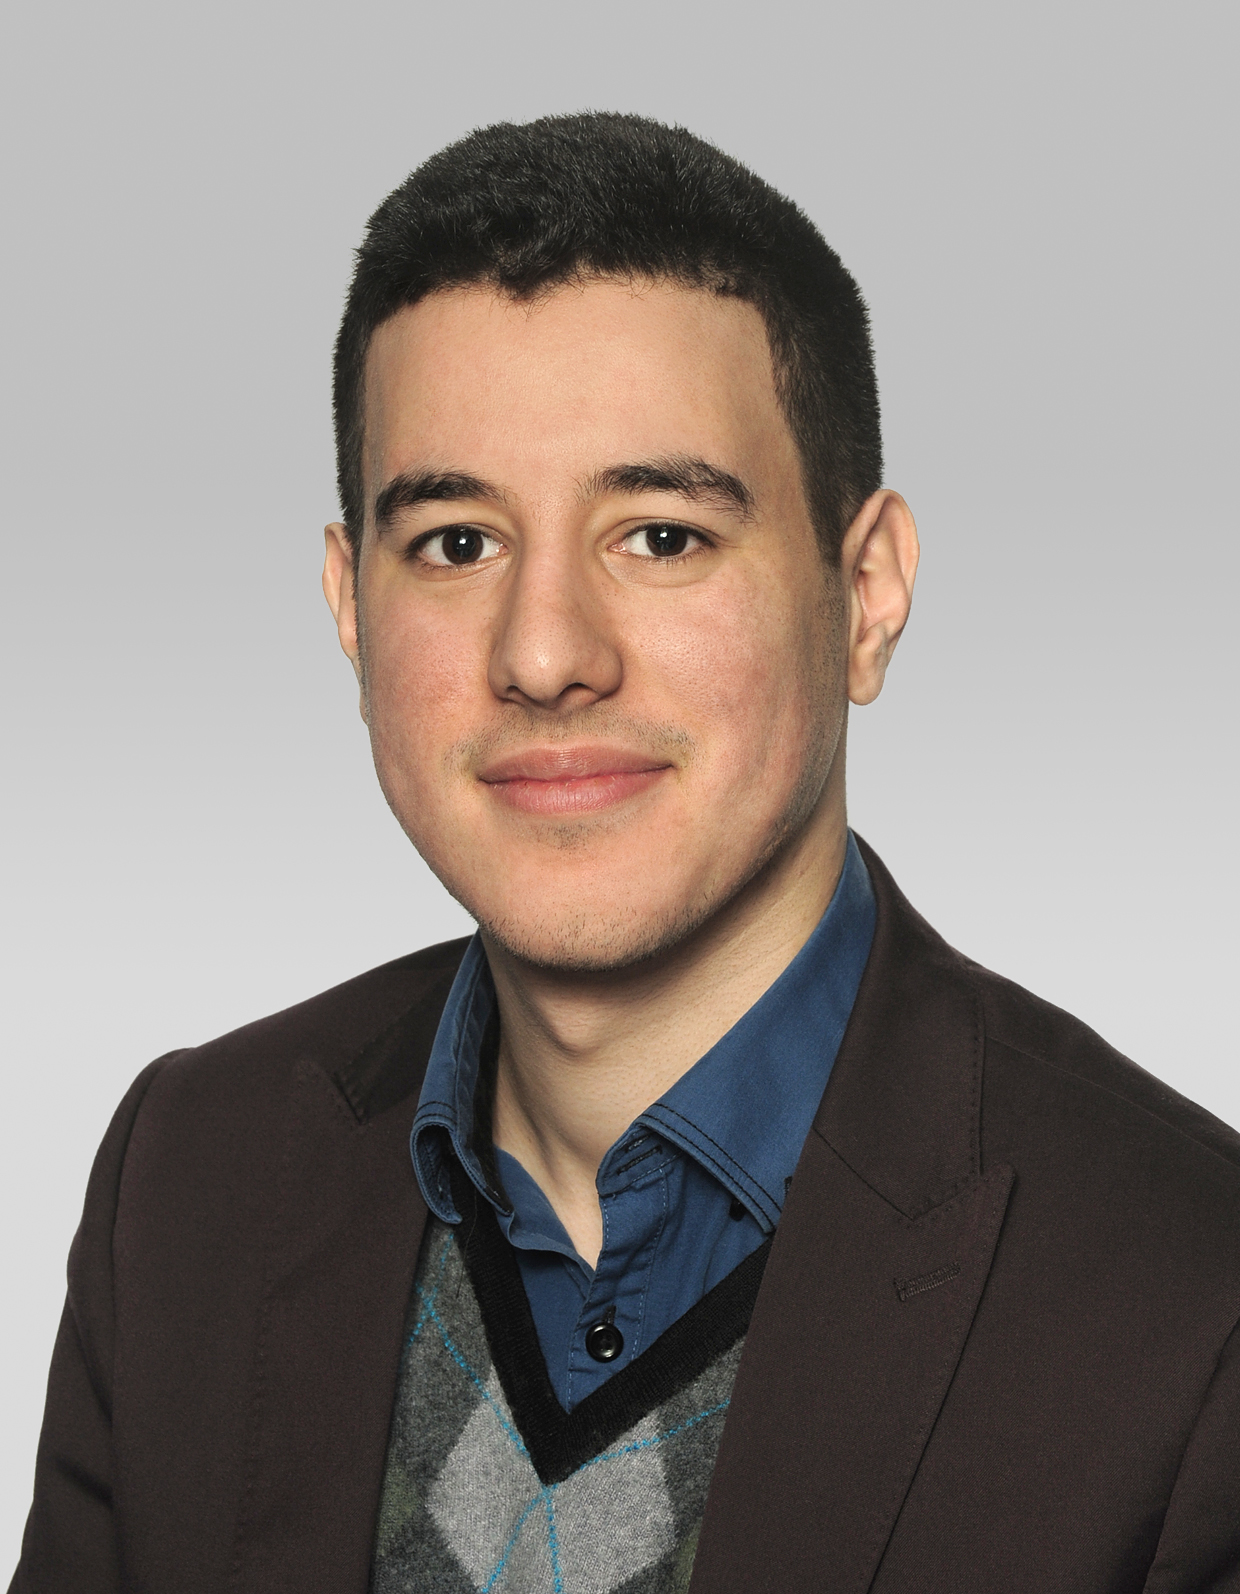
\includegraphics[width=3cm]{Legheraba-Mohamed.jpg}
\end{minipage}
\vspace{-6ex}
% to make maketitle work without begin of page
{\let\newpage\relax\maketitle}
% to remove page number
\thispagestyle{empty}

\vspace{-6ex}

\section*{Formation}
\begin{tabular}{L!{\VRule}R}
\textbf{\textit{2015--2018}} & \textbf{École d'ingénieur Polytech Sorbonne}, spécialité \textit{Mathématiques Appliquées et Informatique Numérique}. Semestre Erasmus aux Pays-Bas (TU Delft) en Hiver 2017.\\[0.75cm]
\textbf{\textit{2013--2015}} & \textbf{École d'ingénieur Polytech Sorbonne}, classe \textit{PeiP} (Préparation aux écoles d'ingénieur Polytech)\\[0.75cm]
\textbf{\textit{2013}}&\textbf{Baccalauréat S}, mention Bien. Lycée Chaptal. \\
\end{tabular}
 

\section*{Expérience Professionnel}
\begin{tabular}{L!{\VRule}R}
\textbf{\textit{Depuis 2019}}&{\bf Développeur Blockchain, Sia Partners}\\[0.25cm]

& \tabitem \textbf{Développement d'applications blockchain pour les clients de Sia Partners} (réseau Corda pour un gestionnaire d'actifs, application mobile de paiement en cryptomonnaie, ...)

\\[0.20cm]
& \tabitem \textbf{Étude des cas d'usages de la blockchain avec les équipes métiers} (traçabilité des aliments, enregistrement des essais cliniques, horodatage des données de capteurs IoT, ...)

\\[0.20cm]
& \tabitem \textbf{Veille R\&D et rédaction d'articles sur la blockchain et les cryptomonnaies} (étude des réseaux blockchain Liquid, Libra et TON, des technologies Lightning Network, Taproot et Multi-Party Computation, étude de l'utilisation de la blockchain pour la gestion des réseaux 5G, ...)

\\[0.20cm]
\textbf{\textit{Mars--Septembre 2018}}&{\bf Stage Veille R\&D, OFI AM, 6 mois}.\\
& Veille autour des technologies de Blockchain, de l’automatisation de tâches avec Airflow, de la conteneurisation d’application avec Docker et de la supervision système avec Tableau Server. \\

\end{tabular}
 
 
\section*{Compétences}
\hspace*{1ex}
\begin{minipage}[ht]{0.50\textwidth}
\textbf{Blockchain}: \textbf{\textit{Bitcoin}}, \textbf{\textit{Ethereum}}, Hyperledger, Corda \\[0.1cm]
\textbf{Smart contracts}: \textbf{\textit{Solidity}}, Bitcoin Script, Chaincodes \\[0.1cm]
\textbf{Outils système}: \textbf{\textit{Shell}}, Linux, Git, Bash, \textbf{\textit{Docker}} \\[0.1cm] 
\textbf{Mathématiques}: Cryptographie, Statistiques, Graphes \\[0.1cm]
\textbf{Protocoles}: \textbf{\textit{Lightning Network}}, IPFS, BitTorrent \\
\end{minipage}
\begin{minipage}[ht]{0.50\textwidth}
\textbf{Bases de données}: MySQL, \textbf{\textit{PostgreSQL}}, Neo4J \\[0.1cm]
\textbf{Programmation}: \textbf{\textit{Python}}, \textbf{\textit{JavaScript}}, C/C++, R \\[0.1cm]
\textbf{Frameworks}: \textbf{\textit{ReactJS}}, \textbf{\textit{Nodejs}}, Flask, PyQt, R Shiny \\[0.1cm]
\textbf{Informatique}: Algorithmique , Parallélisme, Compilateurs \\[0.1cm]
\textbf{Cloud}: Google, AWS, Azure, Gitlab CI/CD, Kubernetes \\
\end{minipage}
\vspace{-5ex}
\section*{Autres expériences}
\begin{tabular}{L!{\VRule}R}
\textbf{\textit{Depuis 2018}} & Association \textbf{Le Trait D’Union}, Aide aux devoirs auprès de lycéens et de collégiens. Rédaction de dossiers de subventions. \\[0.75cm]

\textbf{\textit{2014--2017}} & Association étudiante \textbf{Averroès}, Dons alimentaire pour les étudiants, trésorier puis président. \\
\end{tabular}
\section*{Loisirs}
\hspace*{1ex} Cinéma (films et séries de science-fiction, de fantasy, …) \\
\hspace*{1ex} Histoire (Antiquité et Moyen Âge) \\
\end{document}
